\documentclass{article}

\usepackage{graphicx}
\usepackage{tikz}
\usepackage{tikzsymbols}
\usetikzlibrary{calc,patterns,shapes.geometric}
\pagestyle{empty}
\usepackage[margin=0pt]{geometry}
\geometry{papersize={14in,12in}}

\def\centerarc[#1](#2)(#3:#4:#5){\draw[#1] ($(#2)+({#5*cos(#3)},{#5*sin(#3)})$) arc (#3:#4:#5);}

\begin{document}
	\begin{figure}
		\centering
		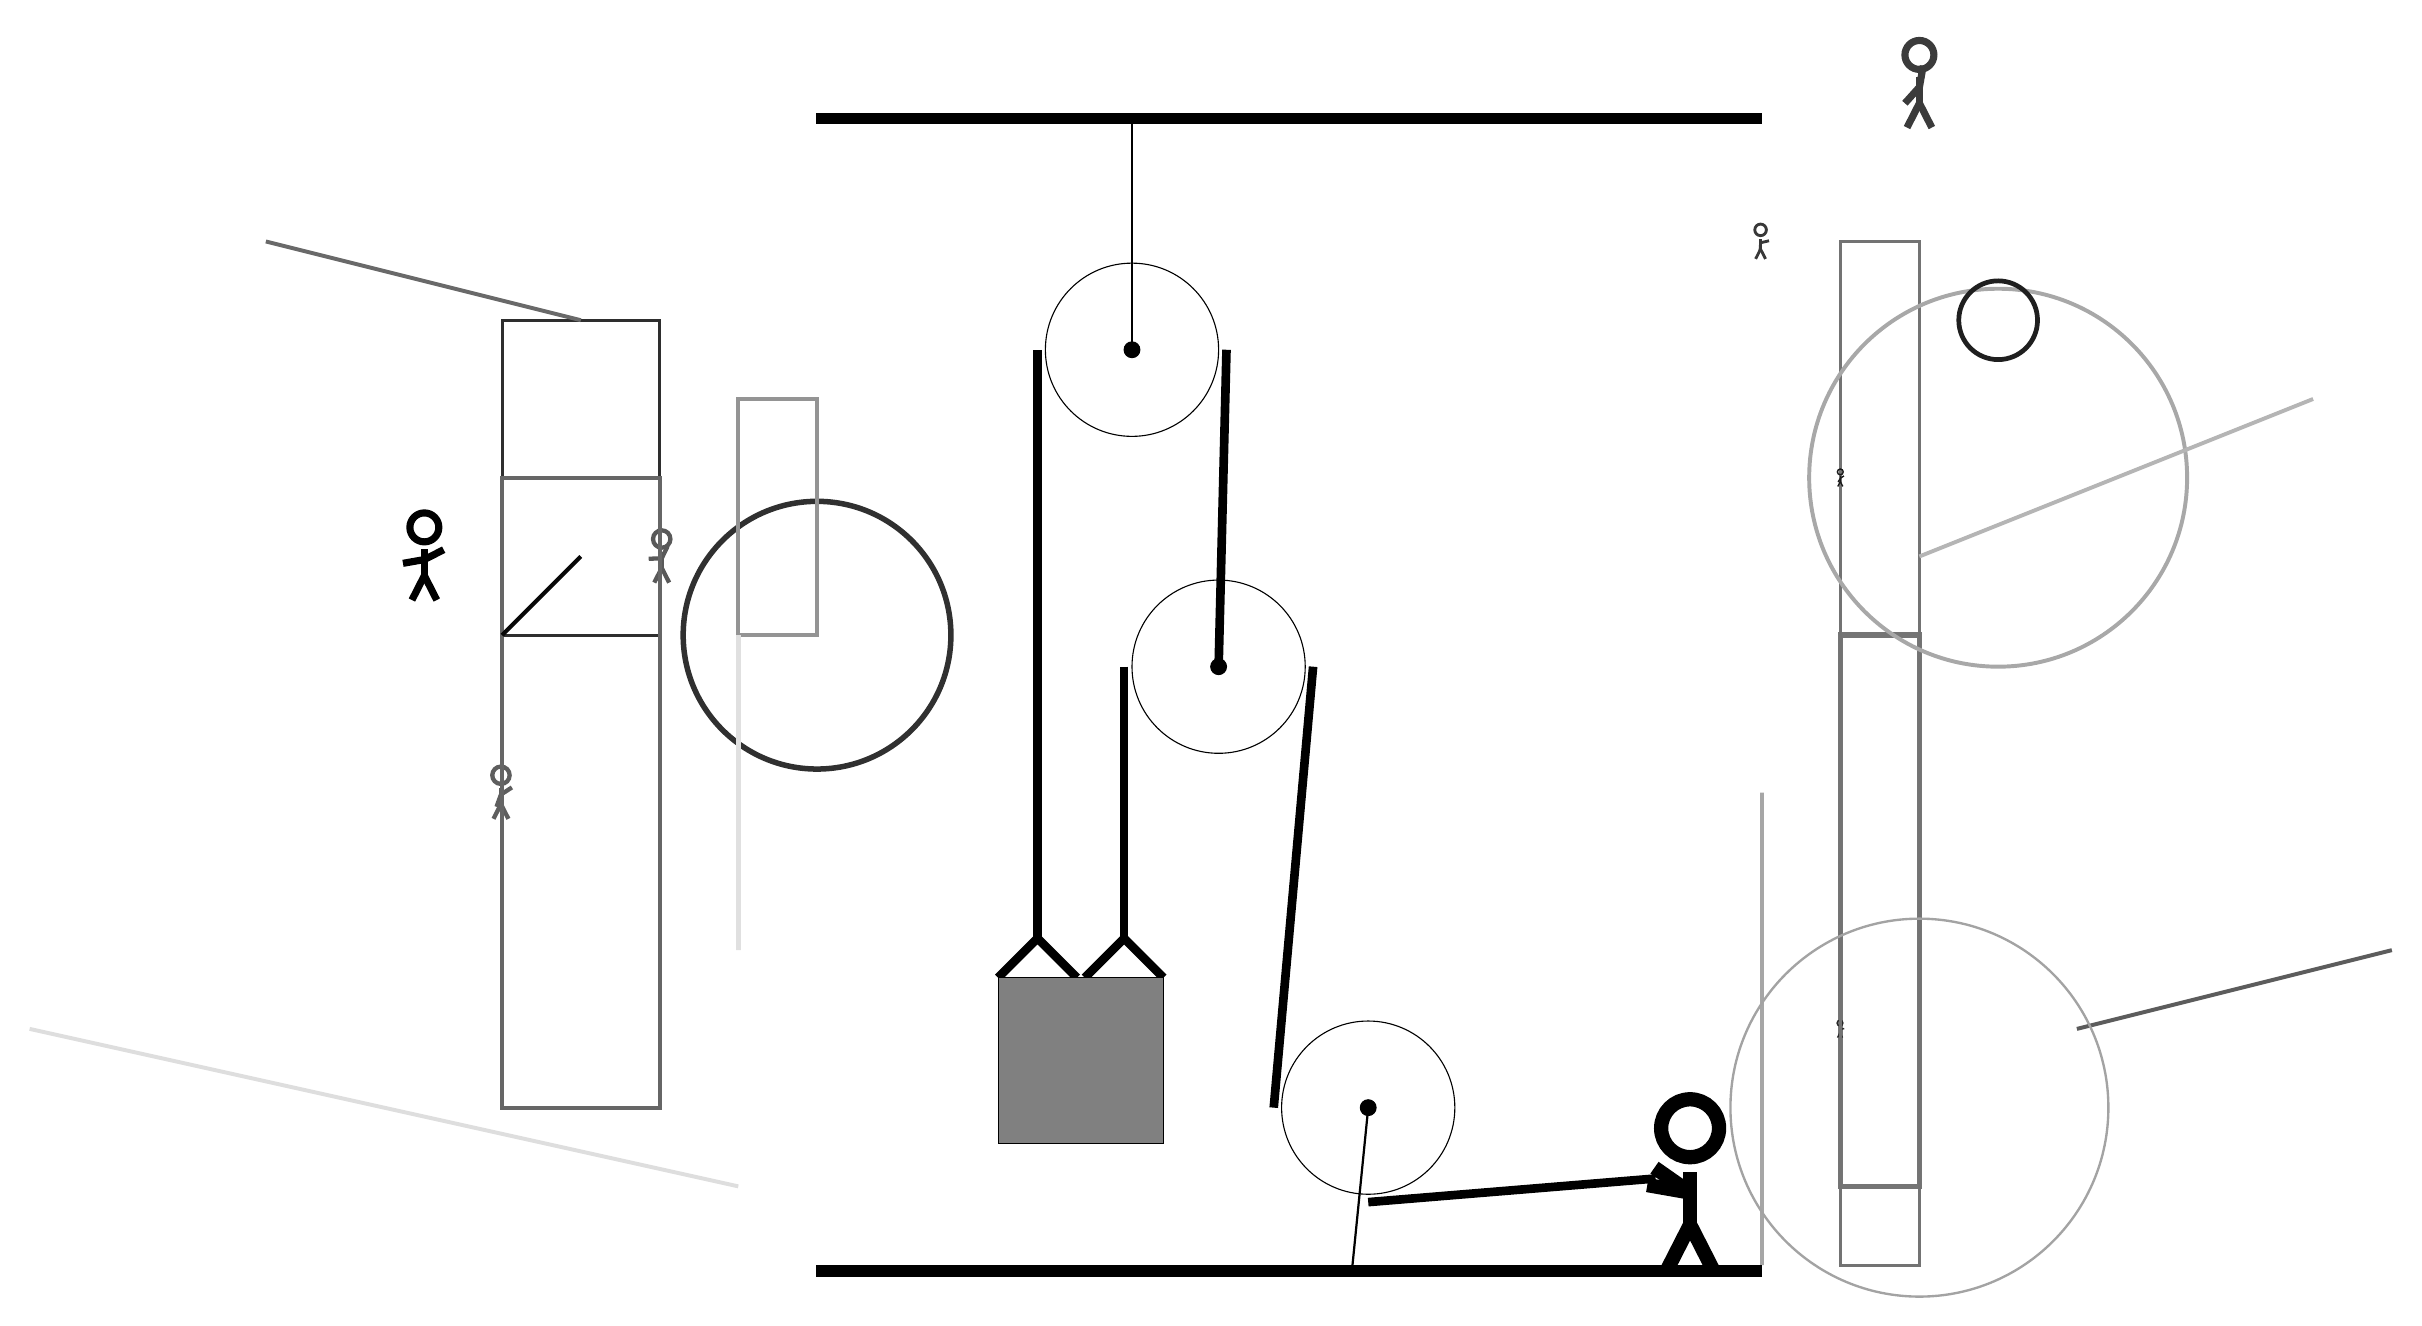
\begin{tikzpicture}
			%%%%% START %%%%%
			
			\draw[fill=black] (-2, 11.5) rectangle (10, 11.625);
			
			\draw[line width=0.4mm, color=black!82] (-4, 9) rectangle (-6, 5);
			
			\draw[line width=0.5mm, color=black!64](14, 0) -- (18, 1);
			\draw[line width=0.5mm, color=black!13](-3, -2) -- (-12, 0);
			\node[line width=0.4mm, color=black!77] at (12, 12) {\Strichmaxerl[5][48][80]};
			\draw[line width=0.7mm, color=black!54] (11, -2) rectangle (12, 5);
			\node[line width=0.3mm, color=black!65] at (-4, 6) {\Strichmaxerl[3][2][64]};
			
			\node[line width=0.2mm, color=black!84] at (11, 0) {\Strichmaxerl[1][85][13]};
			\draw[line width=0.4mm, color=black!55] (11, 10) rectangle (12, -3);
			\draw [line width=0.7mm, color=black!81](-2, 5) circle (1.7);
			\draw [line width=0.5mm, color=black!34](13, 7) circle (2.4);
			\node[line width=0.6mm, color=black!78] at (10, 10) {\Strichmaxerl[2][86][13]};
			\draw[line width=0.5mm, color=black!35] (10, 3) rectangle (10, -3);
			\draw [line width=0.3mm, color=black!36](12, -1) circle (2.4);
			
			\node[line width=0.3mm, color=black!63] at (-6, 3) {\Strichmaxerl[3][70][33]};
			\draw[line width=0.5mm, color=black!59](-5, 9) -- (-9, 10);
			\draw [line width=0.2mm, color=black!18](-9, 2) circle (0.0);
			
			\draw[line width=0.5mm, color=black!60] (-4, 7) rectangle (-6, -1);
			
			\node[line width=0.5mm, color=black!90] at (11, 7) {\Strichmaxerl[1][60][34]};
			\draw[line width=0.5mm, color=black!42] (-2, 8) rectangle (-3, 5);
			\draw [line width=0.6mm, color=black!88](13, 9) circle (0.5);
			\draw[line width=0.6mm, color=black!12] (-3, 1) rectangle (-3, 5);
			
			\node[line width=0.4mm, color=black!100] at (-7, 6) {\Strichmaxerl[5][10][27]};
			
			\draw[line width=0.5mm, color=black!29](12, 6) -- (17, 8);
			\draw[line width=0.5mm, color=black!97](-6, 5) -- (-5, 6);
			
			\draw (2, 8.625) circle (1.1);
			\draw[fill=black] (2, 8.625) circle (0.1);
			\draw[thick] (2, 8.625) -- (2, 11.5);
			
			\draw (3.1, 4.6) circle (1.1);
			\draw[fill=black] (3.1, 4.6) circle (0.1);
			
			\draw (5, -1) circle (1.1);
			\draw[fill=black] (5, -1) circle (0.1);
			\draw[thick] (5, -1) -- (4.8, -3);
			
			\draw[line width = 1.1mm]  (0.3, 0.65) -- (0.8, 1.15) -- (1.3, 0.65);
			\draw[line width = 1.1mm]  (1.4, 0.65) -- (1.9, 1.15) -- (2.4, 0.65);
			\draw[fill=black!50] (0.3, 0.65) rectangle (2.4, -1.45);
			
			\draw[line width = 1.1mm] (0.8, 8.625) -- (0.8, 1.15);
			\centerarc[line width = 1.1mm](2, 8.625)(0:180:1.2000000000000002);
			\draw[line width = 1.1mm] (3.2, 8.625) -- (3.1, 4.6);
			\draw[line width = 1.1mm] (1.9, 4.6) -- (1.9, 1.15);
			\centerarc[line width = 1.1mm](3.1, 4.6)(0:180:1.2000000000000002);
			\draw[line width = 1.1mm] (4.3, 4.6) -- (3.8, -1);
			\centerarc[line width = 1.1mm](5, -1)(180:270:1.2000000000000002);
			\draw[line width = 1.1mm] (5, -2.2) -- (8.65, -1.9);
			
			\node at (9, -2) {\Strichmaxerl[10][-35][170]};
			
			\draw[fill=black] (-2, -3) rectangle (10, -3.15);
			
			%%%%% END %%%%%
		\end{tikzpicture}
	\end{figure}	
\end{document}